\chapter{朴素贝叶斯过滤器的改进}

\section{贝叶斯分类流程}
上章描述了几种贝叶斯算法的原理以及优缺点,本节介绍基于贝叶斯算法的垃圾邮件过滤流程。

1) 收集一定数量的垃圾邮件和正常邮件,建立垃圾邮件集和正常邮件集。

2) 对垃圾邮件集和正常邮件集中的邮件进行内容解析,并提取关键词,

3) 建立两个哈希表分别用于存储垃圾邮件集和正常邮件集中的关键词和出现的次数。

4) 计算处理后的每一个关键词的概率。

5) 对于需要判定的邮件,提取其关键词,计算这些关键词的联合概率。

6) 设定一个判断垃圾邮件的阀值,若计算出的联合概率大于该值,则判定为垃圾邮件。反之,则判定为正常邮件。

\section{贝叶斯邮件过滤器的改进方面}
上节描述了贝叶斯的分类流程,为了更好的用贝叶斯算法进行垃圾邮件过滤,我们在以下几个方面对贝叶斯算法进行改进:

(1)	文本表示

在普通文本分类贝叶斯算法中,文本用词语或者短语表示。因为词语和短语是能代表语意的最小单位。但是在垃圾邮件中,垃圾邮件制造者为了避免被过滤,,采用垃圾变种词语代替垃圾词语。譬如:垃圾词语:法轮功,其变种词语可以是法!!轮===功@。我们采用指纹来表示文本,能够较好的辨别变种词汇,指纹特征会在3.3节中进行详细描述。

(2)	特征选择

普通贝叶斯文本分类算法在特征选择上大多采取信息增益,期望交叉熵等算法。通过对贝叶斯原理的分析,发现特征的分布情况与特征代表类别能力息息相关,因此提出一种新的特征选择方法,基于类条件分布的算法,具体会在第4.4节中给出描述

(3)	 阈值动态调整

朴素bayes通过学习来构造模型参数,其学习过程是一个由浅至深的过程。最开始,学习的样本少,导致模型参数不够精确,判断一封邮件为垃圾邮件的分数也不准确,随着学习的深入,判断的准确性也随之慢慢提高.因此,我们提出阈值动态调整算法,来适应不断提高的邮件类别判断准确性.这部分在3.5节中会有详细描述。

\section{文本表示}
\subsection{词语特征项}
在文本分类领域中,通常采用向量模型(VSM )来表示文本,一篇文本可以表示成为一个n维向量$(t_1,t_2,t_3,...,t_n)$。其中$t_i(i=1,...,n)$表示第i个特征项的权重。

在英文文本中,特征项通常定义为用空格键、制表符或各种标点符号及重音符号等隔开的一系列连续字符串,一般情况下,特征项就是有意义的单词或词组。在字符处理过程中,所有的大写字母转换成小写字母。所有空格键、制表符、换行符和各种标点符号及重音符号都删除掉。

在中文文本中,特征项可以是字、词、短语或者某种概念,在中文文本中主要指经过分词处理后得到的词汇。但是对多封垃圾邮件进行相似度比较的时候,我们发现在同类垃圾邮件出现较高的是一些文本块短语。并且现在的垃圾邮件制造者为了避免被过滤,经常采用垃圾词汇变种的方法来防止被过滤,譬如:在垃圾邮件中经常出现以下变种词语:法¥¥轮\%\%\%\%功,功999产**党的暴———政等等,所以,在日新月异的垃圾邮件变种中,单纯的采用词语特征已经不能满足要求。

\subsection{指纹散列特征项}
指纹应用在相似邮件的比较上。在比较两封邮件是否相似的时候,可以先把两封邮件划分为很多个文本块(实际上也是子字符串),如果两封邮件是相似的,那么它们之间一定包含很多公有的文本块。而且这些文本块之间的比较操作,是精确比较,因此就可以用散列方法来进行优化。在文献[5]中就提出了一个观点:在这种应用场合中,可以用一组散列值来代表一个文件(而不是一个散列值)。这样的一组散列值在以下的论述中就称为邮件的“指纹”。

其中的每一个散列值, 称为指纹的一个元素, 可以从邮件中的一个片断中提取。按照这种思路, 从一封邮件中提取指纹的步骤可以这样进行:

(1) 把一封邮件看作n个文本块的集合;

(2) 引入一个散列函数,计算每个文本块的散列值;

(3) 按照一定规律,筛选出一些散列值,作为这封邮件的特征代码表。或者称为邮件的”指纹”。

这一节中介绍的是一种通用的思路。通过指定不同的文本块划分方法、选用不同的散列函数或者对散列值采用不用的筛选条件,按照上述步骤可以生成多种指纹算法。

\subsection{一种指纹算法}

下面介绍一种用于最初用于文件管理领域的指纹算法。这种算法的效率很高,因此在国外最近的一些反垃圾邮件研究中仍然采用了这种算法。

下面描述指纹的计算过程。

 (1) 文本块的划分。这种算法从文档的每一个位置开始,都取出一度为 k的子字符串。这样在一个长度为 n 的文档中,一共包含n-k+1个这样的字符串。
 
(2) 散列函数采用了Karp-Rabin算法[7]

  Karp-Rabin算法是一种著名的模式匹配算法。它通过把字符串的匹转换成相应的整数的匹配,而大大提高了匹配的效率。这种算法在计算”相应的整数”时,对长度为 k的子字符串 用了以下的散列函数:
\begin{equation}
 H_i=t_i*p^{k-1}+t_{i+1}*p^{k-2}+...t_{i+k-2}*p^+t_{i+k-1} ~~~~~~~~~~~~~~(P\in N)
\end{equation}
如果对每一个子字符串的散列值都从头开始计算,代价是很高的,karp-Rabin算法采用了以下方法来进行简化:
\begin{equation}
 H_{i+1}=p*H_i+t_{i+k} ~~~~~~~~~~~~~~t_i*p^k
\end{equation}

由于$P^k$是一个常数,所以采用了以上的简化方法以后,每个指纹元素 Hi的计算代价就只有两次乘法和加减法各一次,是非常低的。

 上述计算方法得出的指纹元素往往会超过一个整数的表示范围,因此实际应用的时候可以对上述计算结果取模,或取计算结果中最低的几个位。
\section{特征选择}
特征选择是文本分类中的重要研究领域,其目的是要在一个训练文本的众多的特征中选择出能代表该文本及与该文本所属类别的若干重要特征。特征选择考虑的首要问题是特征与类之间的关系,即选择出来的特征是否真正代表一个类。

  常见的特征选择的方法有:期望交叉熵,信息增益法,互信息法。卡方检验法,主成分分析发等。这些方法或者从信息论的角度或者从统计分析的角度,来找出含有信息量最大或者影响显著的特征,而忽略掉其余的特征,达到特征约简的目的。
\subsection{信息增益}
信息增益,是决策树技术中经常采用的一种选择最佳节点的方法。它利用的是信息论中熵的概念。在信息论中,熵是对事物不确定性的一种度量。它是以各个特征取值情况来划定学习样本空间,根据所获得信息增益的多少来选择有效的特征。特征的信息增益如下所示:
\begin{equation}
 IG(t)=\sum_{i=1}^{n}p(c_i)+p(t)\sum_{i=1}^{n}p(c_i|t)\log p(c_i|t)+p(\bar{t})\sum_{i=1}^{n}p(c_i|\bar{t})\log p(c_i|\bar{t})
\end{equation}
其中$p(c_i)$为文档集中出现类别$c_i$的概率;p(t)为特征出现在文档集中的概率;$p(c_i|t)$表示当t出现在文档集中时,文档属于$c_i$的概率;$p(c_i|\bar{t})$表示当t不出现在文档集中时,文档属于$c_i$的概率。

特征在文本中是否出现都将为文本分类提供信息,计算不同情况下的条件概率已确定提供的信息量的大小。信息增益利用特征取值情况划分训练样本空间,根据所获得信息量的多少选择特征。在进行特征选择时,选择信息增益大的那些特征。该特征选择方法存在的问题是如果一个特征在类中出现,而在类中不出现,这个特征本身非常重要,但是对各log值求和之后相抵消,结果为0,与某些词无法区分,解决这个问题有两种方法:一是对log值取绝对值,二是略去log值小于0的情况。此外,该方法计算也比较复杂。

\subsection{实验及分析}
为了比较三种特征选择方法对分类精度的影响,我们对分别采用三种特征选择方法的过滤器采用离线和在线两种过滤模式来进行过滤。其中在线过滤模式在trec07 p 邮件集上进行,并且采用在线立即反馈模式,离线模式在 sewm 2008 公开集上进行。

在特征选择标准上,提取的关键特征的个数对过滤精度也有一定的影响,因此我们分别提取特征数为8,10,15上,并且比较三种特征选择方法在邮件过滤精度上的区别。首先比较在trec07 p上采用在线及时反馈的实验,实验使用TREC 的Spam 评测工具,实验结果如下所示:



\begin{table}[!htbp]
\centering
\begin{tabular}{|p{3cm}|p{3cm}|p{3cm}|p{3cm}|}% 通过添加 | 来表示是否需要绘制竖线
\hline  % 在表格最上方绘制横线
评价参数|特征选择方法&信息增益&期望交叉熵&类条件分布(ccd值)\\
\hline  %在第一行和第二行之间绘制横线
Ham\%&2.39(1.76-3.16)&1.18 (1.05-1.32)&1.42 (0.95-2.05)\\
\hline % 在表格最下方绘制横线
Spam\%&1.10 (0.88-1.35)&0.87 (0.79-0.96)&0.16 (0.09-0.28)\\
\hline % 在表格最下方绘制横线
Lam\%&1.62 (1.37 - 1.91)&1.01 (0.95 - 1.08)&0.48 (0.34 - 0.69)\\
\hline % 在表格最下方绘制横线
1-ROCA\%&0.3509 (0.1166 - 1.0512)&0.3728 (0.1699 – 1.8844)&0.2963 (0.1453 – 1.
4129)\\
\hline % 在表格最下方绘制横线
\end{tabular}
\caption{特征选取个数为8的三种算法在线过滤精度}
\end{table}


\begin{table}[!htbp]
\centering
\begin{tabular}{|p{3cm}|p{3cm}|p{3cm}|p{3cm}|}% 通过添加 | 来表示是否需要绘制竖线
\hline  % 在表格最上方绘制横线
评价参数|特征选择方法&信息增益&期望交叉熵&类条件分布(ccd值)\\
\hline  %在第一行和第二行之间绘制横线
Ham\%&1.16(1.13-1.42)&1.20(1.03-1.29)&1.32(1.05-1.00)\\
\hline % 在表格最下方绘制横线
Spam\%&0.86 (0.75-0.90)&0.86(0.79-0.95)&0.14(0.05-0.26)\\
\hline % 在表格最下方绘制横线
Lam\%&1.02 (0.94 - 1.11)&1.00 (0.93 -1.07)&0.39 (0.35 - 0.44)\\
\hline % 在表格最下方绘制横线
1-ROCA\%&0.2986(0.2673 -0.3444)&0.2739 (0.2563 – 0.3346)&0.1363 (0.1053 – 0.
3129)\\
\hline % 在表格最下方绘制横线
\end{tabular}
\caption{特征选取个数为10的三种算法在线过滤精度}
\end{table}


\begin{table}[!htbp]
\centering
\begin{tabular}{|p{3cm}|p{3cm}|p{3cm}|p{3cm}|}% 通过添加 | 来表示是否需要绘制竖线
\hline  % 在表格最上方绘制横线
评价参数|特征选择方法&信息增益&期望交叉熵&类条件分布(ccd值)\\
\hline  %在第一行和第二行之间绘制横线
Ham\%&2.15(1.56-3.11)&1.17(1.04-1.33)&1.40 (0.97-2.00)\\
\hline % 在表格最下方绘制横线
Spam\%&0.96(0.78-1.24)&0.88(0.78-0.95)&0.88(0.78-0.95)\\
\hline % 在表格最下方绘制横线
Lam\%&1.32(1.27 - 1.85)&1.32(1.27 - 1.85)&1.32(1.27 - 1.85)\\
\hline % 在表格最下方绘制横线
1-ROCA\%&0.3423(0.1166- 1.0512)&0.3423(0.1166- 1.0512)&0.2567(0.1343 – 1.
3879)\\
\hline % 在表格最下方绘制横线
\end{tabular}
\caption{特征选取个数为15的三种算法在线过滤精度}
\end{table}

\newpage
实验结果显示,不论是在线立即反馈还是离线模式,采取同一个邮件过滤算法时,特征选取个数不同,垃圾邮件过滤精度不同。当特征选取个数为10时,不论是使用信息增益,期望交叉熵,还是类条件分布特征选择算法时,其邮件过滤精度要好于特征选取个数为8和15的算法。这表明特征选择的个数并不是越多越好;特征选取多,不仅增加了计算的难度,而且也会带来一些类别代表能力不强,类别模拟两可的噪音特征的加入。又由于文本内容中各个词汇之间本来就不是完全独立的,朴素贝叶斯方法的前提是假设特征之间相互独立,所以当特征值提取数量增加之后,特征值之间相互依赖的机会增加,独立性变小。但是选取的特征太少,使得分类只片面考虑到部分的特征,忽略掉了很多对分类影响大的特征,导致分类准确性降低。

\section{改进的朴素贝叶斯邮件过滤流程}
本章第二节到第六小节描述了对朴素贝叶斯算法的几个方面的改进,本节总结这些改进方法,并将这些改进方法运用到朴素贝叶斯邮件过滤上。 

改进后的朴素邮件过滤算法的流程图如下所示:
\begin{figure}[htbp]
\centering
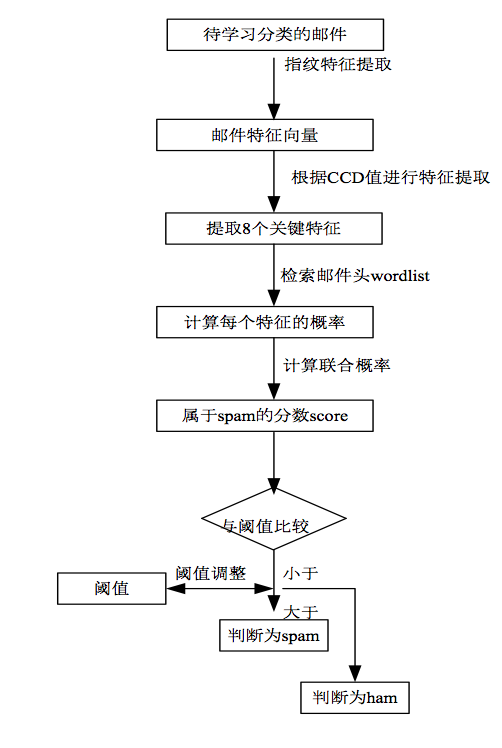
\includegraphics[width=.8\textwidth]{bays7.png}
\caption{改进朴素贝叶斯流程图}
\label{fig:logo}
\end{figure}

\newpage

\begin{lstlisting}[language=python]
<strong>'''''******************************* 
  Copyright (C), 2015-2020, cyp Tech. Co., Ltd. 
  FileName:           朴素贝叶斯实例.cpp 
  Author:             cyp      
  Version :           v1.0           
  Date:               2015-10-21 上午10:38 
  Description:        利用朴素贝叶斯原理对邮件进行分类      
  Function List:       
    1.  createVocalList:计算输入各集的并集,且每个元素是unique 
    2.  setofWords2Vec:  运用词集方式将数据预处理 
    3.  bagofWords2Vec:  运用词袋方式将数据预处理 
    4.  trainNB0:       训练数据 
    5.  classifyNB:      对email进行分类 
    6.  test             相当于主函数,训练模型并测试 
********************************************'''  
  
  
'''''*************************************** 
需要导入的模块 
********************************************''  
import random  
import math  
import numpy as np  
import os  
  
'''''********************************************* 
  Function:        createVocalList 
  Description:     计算输入各集的并集,且每个元素是unique 
  Calls:            
  Called By:       test 
  Input:           dataSet输入的数据集,及单词向量集 
  Return:          返回输入数据集的并集,返回数据的数据类型是list 
                   表示出现过的单词 
************************************************'''  
def createVocalList(dataSet):  
    vocalSet = set([])                  #创建一个空集  
    for data in dataSet:  
        vocalSet = vocalSet | set(data) #利用set的特性求两个集合的并集  
    return list(vocalSet)               #以list的方式返回结果  
      
      
'''''******************************************** 
  Function:        setofWords2Vec 
  Description:     判断的向量的单词是否在词库中是否出现,如果出现 
                   则标记为1,否则标记为0 
  Calls:            
  Called By:       test 
  Input: 
                   vocabList: 
                   词库,曾经出现过的单词集合,即createVocalList 
                   inputSet: 
                   测试的单词向量 
  Return:          returnVec是一个同vocalList同大小的数据,
  如果inputset单词 
                   出现在vocalList则将returnVec对应的位置置1,否则为0 
************************************************'''  
def setofWords2Vec(vocalList,inputset):  
    returnVec = [0]*len(vocalList)         
    #同vocalList同大小的list,开始假设每个单词都没出现,即全为0  
    for word in inputset:                                          
        if word in vocalList:        #如果输入的单词出现在词库中,则置1     
            returnVec[vocalList.index(word)] = 1  
        else:                        #如果没出现在词库中,默认为0,并输出  
            print("the word:%s is not in my Vocabulary!"%word)  
    return returnVec                 #返回结果  
'''''********************************************
  Function:        bagofWords2Vec 
  Description:     统计的单词是否在词库中出现频率 
                  
  Calls:            
  Called By:       test 
  Input: 
                   vocabList: 
                   词库,曾经出现过的单词集合,即createVocalList 
                   inputSet: 
                   测试的单词向量 
  Return:          returnVec是一个同vocalList同大小的数据,对应位置 
                    表示该单词出现的个数 
***********************************************'''  
def bagofWords2Vec(vocalList,inputset):  
    returnVec = [0]*len(vocalList)         
    #同vocalList同大小的list,开始假设每个单词都没出现,即全为0  
    for word in inputset:                                          
        if word in vocalList:        #如果输入的单词出现在词库中,则加1     
            returnVec[vocalList.index(word)] += 1  
    return returnVec                 #返回结果  
'''''****************************************** 
  Function:        trainNB0 
  Description:     统计侮辱性email出现概率,侮辱性邮件各单词出现的概率,非 
                   侮辱性email各单词出现概率 
  Calls:            
  Called By:       test 
  Input: 
                   trainDataSet:参与训练的数据集,
                   即setofWords2Vec返回数据的集合 
                   trainLabels:训练数据的标签 
  Return:           
                    pShame:侮辱性email 
                    p0Vect:非侮辱性email中单词出现的概率 
                    p1Vect:侮辱性email中单词出现的概率 
********************************************'''  
def trainNB0(trainDataSet,trainLabels):  
    numTrains = len(trainDataSet)     #训练数据的组数  
    numWords = len(trainDataSet[0])   #每组训练数据的大小  
    pShame = sum(trainLabels)/float(numTrains)  
    #标签中1表示侮辱,0表示非侮辱,故上述统计侮辱性email出现概率  
    #zeros(numWords)表示1*numWords数组,非numWords*numWords数组  
    #p0Num = np.zeros(numWords)     #存储统计非侮辱性邮件各单词出现频率  
    #p1Num = np.zeros(numWords)         #存储统计侮辱性邮件各单词出现频率  
    #p0SumWords = 0.0                  #非侮辱性邮件中单词总数  
    #p1SumWords = 0.0                  #侮辱性邮件中单词总数  
    #为了防止与0相乘,故初始化为1,因为两者的初始化一样,所以不影响结果  
    p0Num = np.ones(numWords)        #存储统计非侮辱性邮件各单词出现频率  
    p1Num = np.ones(numWords)           #存储统计侮辱性邮件各单词出现频率  
    p0SumWords = 2.0                    #非侮辱性邮件中单词总数  
    p1SumWords = 2.0                    #侮辱性邮件中单词总数  
    for i in range(numTrains):  
        if trainLabels[i]==1:         #如果为侮辱性email  
            p1Num += trainDataSet[i]  #统计非侮辱性邮件各单词  
        else:  
            p0Num += trainDataSet[i]  #统计侮辱性邮件各单词  
    p0SumWords = sum(p0Num)           #计算非侮辱性邮件中单词总数  
    p1SumWords = sum(p1Num)           #计算侮辱性邮件中单词总数  
    p0Vect = p0Num/p0SumWords         #非侮辱性邮件中单词出现的概率  
    p1Vect = p1Num/p1SumWords         #侮辱性邮件中单词出现的概率  
    return pShame,p0Vect,p1Vect  
      
'''''************************************* 
  Function:        classifyNB 
  Description:     对email进行分类 
  Calls:            
  Called By:       test 
  Input: 
              vec2Classify:要分类的数据 
              pShame:侮辱性email 
               p0Vect:非侮辱性email中单词出现的概率 
             p1Vect:侮辱性email中单词出现的概率 
  Return:           
              分类的结果,1表示侮辱性email,0表示非侮辱性email 
********************************************'''  
def classifyNB(vec2Classify,p0Vect,p1Vect,pShame):  
    #由于小数相乘,会有很大误差,故先求对数再相乘  
    temp0 = vec2Classify*p0Vect   
    temp1 = vec2Classify*p1Vect  
    temp00 = []   
    temp11 = []  
    #分步求对数,因为log不能处理array,list  
    for x in temp0:  
        if x>0:  
            temp00.append(math.log(x))   
        else:  
            temp00.append(0)  
    for x in temp1:  
        if x>0:  
            temp11.append(math.log(x))   
        else:  
            temp11.append(0)  
    p0 = sum(temp00)+math.log(1-pShame)  #属于非侮辱性email概率  
    p1 = sum(temp11)+math.log(pShame)    #属于侮辱性email概率  
    if p1 > p0: #属于侮辱性email概率大于属于非侮辱性email概率  
        return 1  
    else:  
        return 0  
  
'''''********************************************* 
  Function:        text2VecOfWords 
  Description:     从email的string中提取单词 
  Calls:            
  Called By:       test 
  Input: 
                   string: email字符串 
  Return:           
                   单词向量 
**********************************************'''  
def text2VecOfWords(string):  
    import re        #正则表达式工具  
    listOfWolds = re.split(r"\W*",string)  
    #分割数据,其分隔符是除单词,数字外任意的字符串   
    return [word.lower() for word in listOfWolds if len(word)>2]  
    #单词不区分大小写,及全部转换为(小写),滤除没用短字符串  
  
'''''*****************************************
  Function:        test 
  Description:     将数据部分用来训练模型,部分用来测试 
  Calls:           text2VecOfWords 
                   createVocalList 
                   trainNB0 
                   classifyNB 
  Called By:       main 
  Input: 
  Return:           
******************************************'''  
def test():  
    emailList = []               #存放每个邮件的单词向量  
    emailLabel = []              #存放邮件对应的标签  
    cwd = "C:\\Users\\cyp\\Documents\\
    sourcecode\\machinelearning\\my__code\\chapter4\\"  
    for i in range(1,26):  
        #读取非侮辱邮件,并生成单词向量  
        wordList = text2VecOfWords(open(cwd+r"email\ham\%d.txt"%i
        ,encoding='Shift_JIS').read())  
        emailList.append(wordList)#将单词向量存放到emailList中  
        emailLabel.append(0)      #存放对应的标签  
        wordList = text2VecOfWords(open(
        cwd+r"email\spam\%d.txt"%i,encoding='Shift_JIS').read())  
        #读取侮辱邮件,并生成单词向量  
        emailList.append(wordList)#将单词向量存放到emailList中  
        emailLabel.append(1)      #存放对应的标签  
    vocabList = createVocalList(emailList)#由所有的单词向量生成词库  
    trainSet = [i for i in range(50)]     #产生0-49的50个数字  
    testIndex = []                        #存放测试数据的下标  
    for i in range(10):                   #从[0-49]中随机选取10个数  
        randIndex = int(random.uniform(0,len(trainSet)))  
                                          #随机生成一个trainSet的下标  
        testIndex.append(trainSet[randIndex])#提取对应的数据作为训练数据  
        del(trainSet[randIndex])    #删除trainSet对应的值,以免下次再选中  
    trainDataSet = []             #存放训练数据(用于词集方法)  
    trainLabels = []              #存放训练数据标签(用于词集方法)  
    trainDataSet1 = []             #存放训练数据(用于词袋方法)  
    trainLabels1 = []              #存放训练数据标签(用于词袋方法)  
    for index in trainSet:        #trainSet剩余值为训练数据的下标  
        trainDataSet.append(setofWords2Vec(vocabList,emailList[index]))  
        #提取训练数据  
        trainLabels.append(emailLabel[index])  
        #提取训练数据标签  
        trainDataSet1.append(bagofWords2Vec(vocabList,emailList[index]))  
        #提取训练数据  
        trainLabels1.append(emailLabel[index])  
        #提取训练数据标签  
    pShame,p0Vect,p1Vect = trainNB0(trainDataSet,trainLabels)
    #开始训练  
    pShame1,p0Vect1,p1Vect1 = trainNB0(trainDataSet1,trainLabels1)
    #开始训练  
    errorCount = 0.0          #统计测试时分类错误的数据的个数  
    errorCount1= 0.0          #统计测试时分类错误的数据的个数  
    for index in testIndex:  
        worldVec = setofWords2Vec(vocabList,emailList[index])
        #数据预处理  
        #进行分类,如果分类不正确,错误个位数加1  
        if classifyNB(worldVec,p0Vect,p1Vect,pShame) 
        != emailLabel[index]:  
            errorCount += 1  
        worldVec = bagofWords2Vec(vocabList,emailList[index])
        #数据预处理  
        #进行分类,如果分类不正确,错误个位数加1  
        if classifyNB(worldVec,p0Vect1,p1Vect1,pShame1) 
        != emailLabel[index]:  
            errorCount1 += 1  
    #输出分类错误率  
    print("As to set,the error rate is :",
    float(errorCount)/len(testIndex))  
    print("AS to bag,the error rate is :",
    float(errorCount1)/len(testIndex))  
      
'''''************************************ 
  Function:       main 
  Description:    运行test函数 
  Calls:          test 
  Called By:        
  Input: 
  Return:           
*******************************************'''  
if __name__=="__main__":  
    test()</strong>  

\end{lstlisting}

\section{本章小节}
本章首先介绍了朴素贝叶斯算法的分类流程,并且针对其分类流程提出了四个方面的改进在文本表示方面提出了指纹特征;在概率计算方面提出了新的联合概率公式和解本章首先介绍了朴素贝叶斯算法的分类流程,并且针对其分类流程提出了四个方面的改进在文本表示方面提出了指纹特征;在概率计算方面提出了新的联合概率公式和解


